\begin{figure}[htbp]
\section*{ KDM6A}
\centering
\begin{subfigure}[b]{0.95\textwidth}
\centering
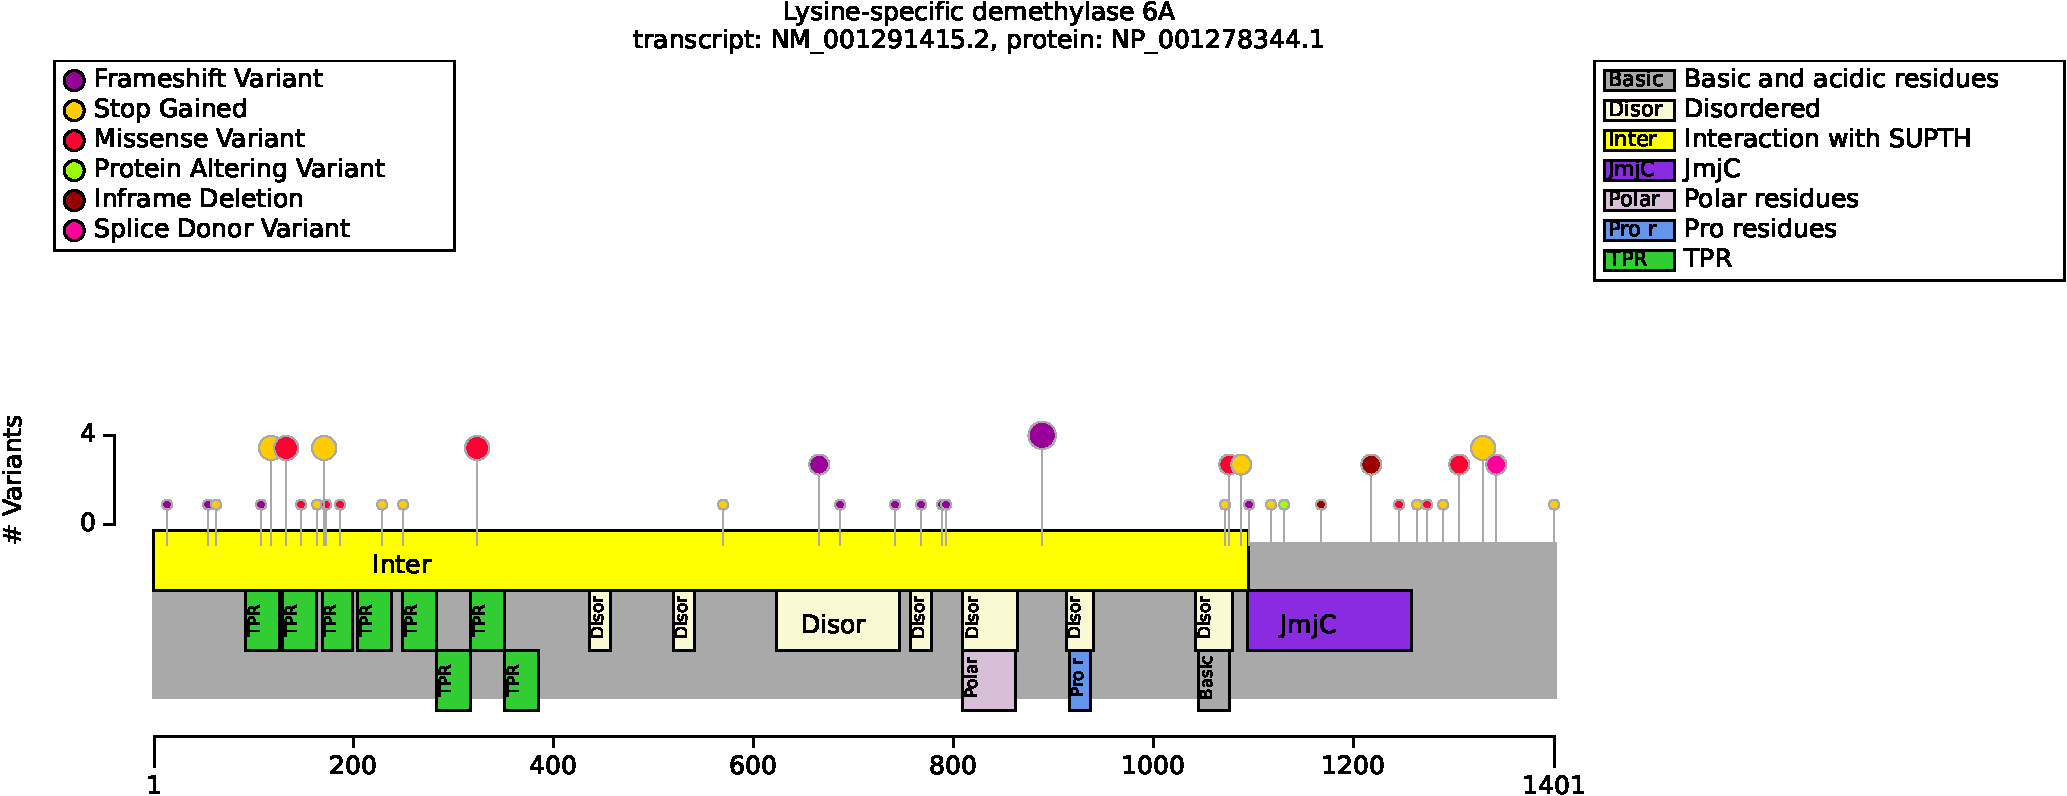
\includegraphics[width=\textwidth]{ img/KDM6A_protein_diagram.pdf} 
\captionsetup{justification=raggedright,singlelinecheck=false}
\caption{Distribution of variants in KDM6A}
\end{subfigure}

\vspace{2em}

\begin{subfigure}[b]{0.95\textwidth}
\centering
\resizebox{\textwidth}{!}{
\begin{tabular}{llllrr}
\toprule
HPO term & FEMALE & MALE & p-value & adj. p-value\\
\midrule
Intellectual disability, severe [HP:0010864] & 7/25 (28\%) & 14/18 (78\%) & 0.002 & 0.008\\
\bottomrule
\end{tabular}
}
\captionsetup{justification=raggedright,singlelinecheck=false}
\caption{Fisher Exact Test performed to compare HPO annotation frequency with respect to FEMALE and MALE. Total of 4 tests were performed. A similar sex difference was reported in ref. \cite{PMID_33674768}.}
\end{subfigure}
\vspace{2em}
\begin{subfigure}[b]{0.95\textwidth}
\centering
\resizebox{\textwidth}{!}{
\begin{tabular}{llllrr}
\toprule
HPO term & p.Asn891ValfsTer27 & Other & p-value & adj. p-value\\
\midrule
Pulmonic stenosis [HP:0001642] & 2/2 (100\%) & 0/59 (0\%) & $5.46\times 10^{-4}$ & 0.016\\
\bottomrule
\end{tabular}
}
\captionsetup{justification=raggedright,singlelinecheck=false}
\caption{         Fisher Exact Test performed to compare HPO annotation frequency with respect to p.Asn891ValfsTer27 and Other. Total of
        29 tests were performed. }
\end{subfigure}
\vspace{2em}
\begin{subfigure}[b]{0.95\textwidth}
\centering
\resizebox{\textwidth}{!}{
\begin{tabular}{llllrr}
\toprule
Genotype (A) & Genotype (B) & total tests performed & significant results\\
\midrule
missense & other & 47 & 0\\
SV & other & 47 & 0\\
\bottomrule
\end{tabular}
}
\captionsetup{justification=raggedright,singlelinecheck=false}
\caption{             Fisher Exact Test performed to compare HPO annotation frequency with respect to genotypes. }
\end{subfigure}

\vspace{2em}

\caption{ The cohort comprised 81 individuals (46 females, 35 males). A total of 87 HPO terms were used to annotate the cohort. Disease diagnosis: Kabuki syndrome 2 (OMIM:300867). . A total of 53 unique variant alleles were found in \textit{KDM6A} (transcript: \texttt{NM\_001291415.2}, protein id: \texttt{NP\_001278344.1}).}
\end{figure}
